\subsection{Implementation}

\begin{frame}{Difficulties}
	Each Worker has its distinct memory and therefore, 
	\begin{itemize}
		\item data needs to be transferred between workers
		\item \dots as well as all functions executed in background threads
	\end{itemize}
	
	\vfill
	
	\begin{block}{Comparsion to other Languages}
		Other languages, e.g. Java, have a shared memory that is accessible by all threads. However, 
			parallelization in JavaScript is more like multiprocess programming using inter process communication.
	\end{block}
\end{frame}

\begin{frame}{Two Possibilities}
	\begin{itemize}
		\item Runtime Serialization of Functions
		\item Transpilation of Source Code
	\end{itemize}
\end{frame}

\begin{frame}{Runtime Serialization of Functions - Overview}
	\begin{center}
		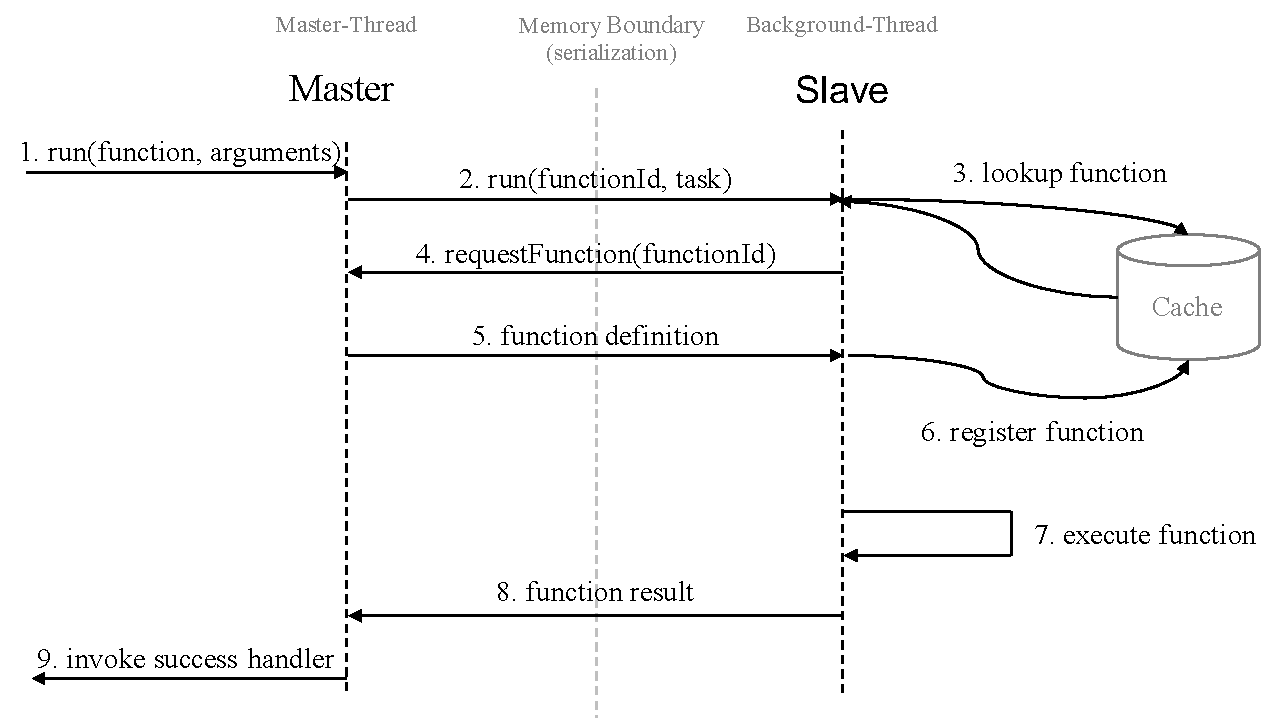
\includegraphics[width=0.8\textwidth]{runtime-system}
	\end{center}
\end{frame}

\begin{frame}[fragile, shrink]{Runtime Serialization of Functions - Serialization}
	\begin{javascriptcode}
const s = func.toString();
const name = getFunctionName(func);
const args = s.substring(s.indexOf("(") + 1, s.indexOf(")")).split(",");
const body = s.substring(s.indexOf("{") + 1, s.lastIndexOf("}")).trim();

const definition = {
	argumentNames: args.map(arg => arg.trim()),
	body,
	id,
	name: name ? name : undefined
};
\end{javascriptcode}

\end{frame}

\begin{frame}[fragile, shrink]{Runtime Serialization of Functions - Deserialization}
	\begin{javascriptcode}
if (definition.name) {
	const args = definition.argumentNames.join(", ");
	const source = `return function ${definition.name} (${args}) { 
		${definition.body} 
	};`; 
	const wrapper = Function.apply(undefined, [ source ]);
	return wrapper();
}
	
return Function.apply(undefined, [
	...definition.argumentNames, 
	definition.body
]);	
\end{javascriptcode}
\end{frame}

\begin{frame}{But what about a Function's Closure?}
\begin{itemize}
	\item Transitive Functions
	\item \dots or Variables referenced from the Function's outer Scope
\end{itemize}

are not supported by Runtime Serialization

\vfill 

\begin{block}{Why Not?}
It's possible to analyze a function at runtime, e.g. by using Babel. However, there is no way to get access to the values of a function's closure as it is the case in C\#. 	
\end{block}
\end{frame}

\begin{frame}[fragile, shrink]{The Issue with Function Closures and Runtime Serialization}
	\begin{columns}[t]
	\begin{column}{0.5\textwidth}
		\begin{block}{UI-Thread}
		\begin{javascriptcode*}{highlightlines={9, 11}, fontsize=\tiny}
const width = 10000;
const height = 10000;

function computePixel(x, y) {
	// ...
}

function computeMandelbrotLine(y) {
	const l = new Uint8ClampedArray(width * 4);
	for (let x = 0; x < width; ++x) {
		l[x * 4] = computePixel(x, y);
	}
	return l;
}

parallel
	.range(height) 
	.map(computeMandelbrotLine)	 
	.then(result => /* handle overall result */);
	\end{javascriptcode*}
	\end{block}
	\end{column}
	\pause
	\begin{column}{0.5\textwidth}
		\begin{block}{Worker-Thread}
			\begin{javascriptcode*}{fontsize=\tiny, highlightlines={2, 4}}
function computeMandelbrotLine(y) {
	const l = new Uint8ClampedArray(width * 4);
	for (let x = 0; x < width; ++x) {
		l[x * 4] = computePixel(x, y);
	}
	return l;
}	
			\end{javascriptcode*}

		\end{block}
		
		\begin{alertblock}{Issue}
			\javascriptinline/height/ variable and \javascriptinline/computePixel/ function are not defined in worker-thread.
		\end{alertblock}
	\end{column}
\end{columns}
\end{frame}

\begin{frame}{Source Code Transpilation}
	\begin{itemize}
		\item Analyses all calls to \javascriptinline/parallel/
		\item Extracts passed functions 
		\item \dots and as well transitive functions
		\item Registers these functions in the background-thread source file
		\item Split into a Babel (extraction) and Webpack-Plugin (registration)
	\end{itemize}
\end{frame}

\begin{frame}[fragile, shrink]{Transpiled Code of Mandelbrot Example}
\begin{columns}[t]
	\begin{column}{0.5\textwidth}
		UI-Thread
		\begin{javascriptcode*}{highlightlines={8-10, 20-24}, fontsize=\tiny}
const width = 10000;
const height = 10000;

function computePixel(x, y) {
	// ...
}

function _environmentExtractor() { 
	return { width: width };
}

function computeMandelbrotLine(y) {
	const l = new Uint8ClampedArray(width * 4);
	// ...
	return l;
}

parallel
	.range(height)
	.inEnvironment(_environmentExtractor()) 
	.map({ 
		identifier: "static:_entrycomputeMandelbrotLine",
		_______isFunctionId: true
	}) 
	.then(result => console.log(result));
\end{javascriptcode*}
	\end{column}
	\begin{column}{0.5\textwidth}
	Worker-Thread
	\begin{javascriptcode*}{highlightlines={1, 2, 6, 12, 22-27}, fontsize=\tiny}
var width;
function computePixel(x, y) { 
	// ...
}

function computeMandelbrotLine(y) { 
	var l = new Uint8ClampedArray(width * 4);
	// ..
	return l;
}
 
function _entrycomputeMandelbrotLine() { 
	try {
		var _environment = arguments[arguments.length - 1];
		width = _environment.width; 
		return computeMandelbrotLine.apply(this, arguments); 
	} finally {
		width = undefined;
	}
} 

slaveFunctionLookupTable.registerStaticFunction({
		identifier: 'static:_entrycomputeMandelbrotLine',
		_______isFunctionId: true
	}, _entrycomputeMandelbrotLine);
\end{javascriptcode*}
	\end{column}
\end{columns}


\end{frame}